\documentclass[12pt, a4paper, openany]{book}
\usepackage{../generalStyle}

\graphicspath{ {./img/} }

\begin{document}

\title{APS - Analisi e Progettazione del Software}

\author{
    Elia Ronchetti\\
	\small{\href{https://t.me/ulerich}{@ulerich}}
}

\date{2022/2023}

\maketitle

\tableofcontents

\chapter*{Introduzione}

Questi appunti di Analisi Matematica sono stati fatti con l'obiettivo di riassumere tutti (o quasi) gli argomenti utili per l'esame di Analisi Matematica del corso di Informatica dell'Università degli Studi di Milano Bicocca.
\\Come fonte ho utilizzato:
\begin{itemize}
	\item Appunti di altri studenti.
	\item Libro "Analisi Uno, teoria ed esercizi" di Giuseppe De Marco (terza edizione).
	\item Esercitazioni in aula della professoressa Susanna Caimi.
\end{itemize}
\section*{Il Corso}
Come già detto, questi appunti sono in funzione del corso di Analisi Matematica di UNIMIB, a.a. 2021/22, insegnato dalla Professoressa Pini.
\subsection*{Programma del corso}
\begin{enumerate}
	\item Numeri Reali
	      \begin{enumerate}
		      \item Funzioni elementari
		      \item Generalità sulle funzioni
		      \item Funzioni reali di una variabile
	      \end{enumerate}
	\item Successioni
	      \begin{enumerate}
		      \item Limiti di successioni reali
		      \item Principio di Induzione
		      \item Limiti notevoli
	      \end{enumerate}
	\item Limiti e continuità
	      \begin{enumerate}
		      \item Limiti di Funzioni
		      \item Limiti notevoli
		      \item Funzioni continue
		      \item Proprietà globali delle funzioni continue
	      \end{enumerate}
	\item Calcoli differenziale
	      \begin{enumerate}
		      \item Derivate di una funzione
		      \item Proprietà delle funzioni derivabili
		      \item Funzioni convesse e concave
		      \item Formula di Taylor
		      \item Grafici di funzioni
	      \end{enumerate}
	\item Calcolo integrale
	      \begin{enumerate}
		      \item Funzioni integrabili secondo Rienmann
		      \item Teorema fondamentale del calcolo e integrali indefiniti
		      \item Metodi d'integrazione
	      \end{enumerate}
	\item Serie numeriche
	      \begin{enumerate}
		      \item Serie, convergenza, convergenza assoluta
		      \item Serie a termini positivi
		      \item Serie a termini di segno variabile
	      \end{enumerate}
\end{enumerate}

\subsection*{Prerequisiti}
\begin{itemize}
	\item \emph{Algebra elementare}: Calcolo letterale, equazioni e disequazioni di primo e secondo grado
	\item \emph{Trigonometria elementare}
	\item \emph{Esponenziali e logaritmi}
\end{itemize}


\chapter{Analisi dei requisiti}
\section{Ideazione}
La maggior parte dei progetto richiede un breve passo iniziale in cui
si esaminano i seguenti tipi di domande:
\begin{itemize}
    \item Il progetto è fattibile?
    \item Comprare e/o costruire?
    \item Stima approssimativa e non affidaivbile dei costi
    \item Dovremmo procedere o fermarci?
\end{itemize}
L'ideazione non è la fase dei requisiti.
\\ Il problema principale che risolve l'ideazione è il seguente:
\begin{center}
    \textbf{Le parti interessate hanno un accordo di base, sulla visione
    del progetto, e vale la pena di investire un'indagine seria?}
\end{center}
Lo scopo è quindi quello di stabilire una visione comune per gli obiettivi del progetto
e capire se questo è fattibile.
\\ In questa fase non si utilizza molto UML (verrà utilizzato soprattutto durante
 l'elaborazione).
\paragraph*{Non hai capito l'ideazione se}
\begin{itemize}
    \item Dura più di qualche settimana
    \item Provi a definire molti requisiti
    \item Ci si aspetta che i piani e le stime siano affidabili
    \item I nomi di molti attori e casi d'uso non sono stati identificati
    \item Troppi casi d'uso sono stati scritti nel dettaglio
    \item Nessun caso d'uso è stato scritto in dettaglio
\end{itemize}
\section{Che sono sono i requisiti}
Un requisito è una capacità o una condizione a cui il sistema e più in generale il
progetto, deve essere conforme.
\\ I requisiti sono un aspetto veramente molto importante, si evidenzia
addirittura che 34 \% delle cause dei fallimenti dei progetti software
riguardano l'attività dei requisiti.
\paragraph*{Ci sono due tipi principali di requisiti}
\begin{itemize}
    \item Requisiti funzionali (comportamentali) - Descrivono il comportamento del
    sistema, in termini di funzionalità fornite ai suoi utenti e informazioni
    che il sistema deve gestire
    \item Requisiti non funzionali (tutti gli altri requisiti) - Sono relativi
    a proprietà del sistema nel suo complesso come per esempio sicurezza, presetazioni,
    scalabilità, usabilità...
\end{itemize}
\subsection{Requisiti funzionali}
Sono funzionalità o servizi che il sistema deve fornire, risposte che l'utente
aspetta dal software in determinate condizioni, risultati che il software deve produrre
in risposta a specifici input.
\paragraph{Il problema dell'imprecisione nella specifica dei requisiti}
Requisiti ambigui possono portare a diverse interpretazioni da sviluppatori e utenti.
In linea di principio i requisiti dovrebbero essere completi e coerenti, quindi
includere la definizione di tutti i servizi richiesti e non essere ambigui.
\subsection{Requisiti non funzionali}
questi definiscono le proprietà e i vincoli del sistema, ad esempio affidabilità,
tempi di risposta, oppure vincoli come la capacità dei dispositivi I/O,
le rappresentazioni dei dati nelle interfacce di sistema, ecc.
\\I requisiti funzionali possono essere più critici dei requisiti funzionali, in caso
contrario il sistema potrebbe risultare inutilizzabile.
\paragraph*{Obiettivi e requisiti} I requisiti non funzionali possono essere molto
difficili da stabilire con precisioni e requisiti imprecisi possono essere
difficili da verificare.
\\ Un obiettivo può essere un intenzione generale dell'utente come la facilità d'uso,
mentre un requisito non funzionale verificabile è una dichiarazione che utilizza
alcune misure oggettivamente verificabili.
Gli obiettivi sono utili agli sviluppatori in quanto trasmettono le intenzioni degli
utenti del sistema.
\paragraph*{Metriche per specificare i requisiti non funzionali}
\begin{center}
    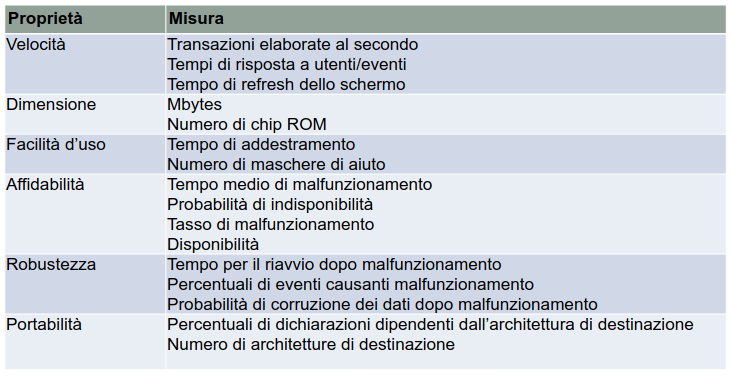
\includegraphics[width=100mm, scale=0.5]{metriche_requisiti_non_funzionali.png}
\end{center}


\chapter{Diagrammi di Sequenza di sistema}


\chapter{Progettazione orientata agli oggetti}
Fino ad ora attraverso l'analisi dei requisiti e l'analisi a oggetti ci siamo
interessati all'imparare a fare la cosa giusta, mentre il lavoro successivo
è fare la cosa bene, attraverso \textbf{la progettazione}.
\\ Ricordiamoci sempre che non dobbiamo prevedere tutto all'inizio (anche perchè
spesso è impossibile), ma dobbiamo necessariamente provocare il cambiamento
all'inizio del progetto per poter scoprire e modificare alcuni requisiti di progettazione
e implementazione. I \textbf{metodi iterativi ed evolutivi} esistono per questo,
abbracciano il cambiamento. Si cerca però di provocare i cambiamenti maggiori nelle
fasi iniziali per avere obiettivi più stabili per le iterazioni successive.
\chapter{Architettura Logica}
Siamo passati da un lavoro di analisi ad un lavoro di progettazione, si inizia
quindi a pensare su larga scala. La progettazione di un tipico sistema
orientato agli oggetti è basata su diversi \textbf{strati architetturali},
come per esempio uno strato per l'interfaccia utente, uno per la logica applicativa, ecc.
\section{Che cos'è l'architettura logica}
L'\textbf{architettura logica} di un sistema software è l'organizzazione su larga scala
delle classi software in package (o namespace), sottoinsiemi e strati.
\\ Uno stile comune per la l'architettura logica è l'\textbf{l'architettura a strati}.
\subsection{Architettura a strati}
Uno strato è un gruppo a grana molto grossa di classi, package o sottosistemi, che ha
delle responsabilità coese rispetto a un aspetto importante del sistema.
\\ Gli strati sono organizzati in modo gerarchico, quelli più alti ricorrono a 
servizi degli strati più bassi (normalmente non avviene il contrario).
\\ Gli strati normalmente comprendono
\begin{itemize}
    \item Presentazione - interfaccia utente
    \item Logica applicativa o strato del dominio - elementi che rappresentano concetti
    del dominio
    \item Servizi tecnici
\end{itemize}
\paragraph*{Due tipi di architettura a strati}
\begin{itemize}
    \item Stretta - uno strato può richiamare solo i servizi dello strato
    immediatamente sottostante
    \item Rilassata - uno strato può richiamare i servizi di strati più bassi di diversi
    livelli
\end{itemize}
Noi ci concentreremo sullo \textbf{strato della logica applicativa (o strato del dominio)}.
\section{Che cos'è un'architettura software}
\begin{itemize}
    \item L'insieme delle decisioni significative sull'organizzazione di un sistema
    software
    \item La scelta degli elementi strutturali da cui è composto il sistema e delle
    relative interfacce
    \item La specifica della collaborazione tra gli elementi strutturali
    \item La composizione di questi elementi strutturali e comportamentali in sottosistemi via
    via più ampi
    \item Lo stile architetturale che guida questa implementazione
\end{itemize}
L'architettura software ha a che fare con la larga scala.
\section{Diagrammi dei Package}
L'architettura logica può essere illustrata mediante un diagramma dei package
di UML, dove uno strato può essere modellato come un package UML.
Un package UML può ragguppare qualunque cosa (classi, altri package, casi d'uso).
\begin{itemize}
    \item \'E molto comune l'annidamento di package
    \item Per mostrare la dipendenza tra i package viene utilizzata una dipendenza UML
    \item Un package UML rappresenta un namespace, in questo modo è possibile
    definire due classi con lo stesso nome su package diversi
\end{itemize}
\subsection{Progettzione degli strati}
Organizzare l astruttura logica di un sistema in strati separati con responsabilità
distine e correlate, con una separazione netta e coesa degli interessi:
Come detto in precedenza:
\begin{itemize}
    \item Gli strati inferiori sono servizi generali e di basso livello
    \item Gli strati superiori sono più specifici per l'applicazione
\end{itemize}
Collaborazione e accoppiamenti vanno dagli strati più alti a quelli più bassi.
L'obiettivo è suddividere un sistema in un insieme di elementi software che
per quanto possibile, possano essere sviluppati e modificati ciascuno
\textbf{indipendentemente dagli altri}.
Nella slide 16 viene riportato un esempio di scelta comune per gli strati,
qui di seguito il link per la slide: \href{https://elearning.unimib.it/pluginfile.php/1463482/mod_resource/content/2/08_Dai%20requisiti%20alla%20progettazione%20e%20architettura%20logica.pdf}{Link slide} 
\subsection*{Vantaggi dell'uso a strati}
La sperazione provocata dall'utilizzo degli strati crea diversi vantaggi fra cui:
\begin{itemize}
    \item riduce l'accoppiamento e le dipendenze, migliora la coesione, aumenta la possibilità di riuso e aumenta
    la chiarezza.
    \item La complessità relativa a questi aspetti è incapsulata e può essere
    decomposta
    \item alcuni strati possono essere sostituiti da nuove implementazioni
    \item Gli strati più bassi contengono funzioni riusabili
    \item Alcuni strati possono essere distribuiti
    \item Lo sviluppo del team è favorito dalla segmentazione logica     
\end{itemize}
\subsection*{Responsabilità coese e seperazione degli interessi}
In uno strato le responsabilità degli oggetti devono essere fortemente coese
l'uno all'altro e non devono essere mescolate con le responsabilità degli altri
strati.
\section{Oggetti e logica applicativa}
Un oggetto software è un oggetto con nomi e informazioni simili al dominio
del mondo reale e assegnare ad esso responsabilità della logica applicativa, un oggetto
di questo tipo è chiamato un oggetto di dominio.
\\ Rappresenta una cosa nello spazio del dominio del problema e ha una logica applicativa
o di business correalata.
\\ Progettando gli oggetti in questo modo si arriva a uno strato della logica
applicativa che può essere chiamato \textbf{strato del dominio} dell'architettura
\subsection{Definizione livelli, trati e partizioni}
\begin{itemize}
    \item Livello (tier): solitamente indica un nodo fisica di elaborazione 
    \item Strato (layer): una sezione verticale dell'architettura
    \item Partizione (partition): una divisione orizzontale di sottosistema di uno strato
\end{itemize}
\subsection{Principio di separazione Modello-Vista}
Gli oggetti di dominio (modello) non devono essere connessi o accoppiati direttamente agli
oggetti UI (vista).
\\ Un rilassamento legittimo di questo principio è il \textbf{Pattern Observer},
qua gli oggetti del dominio inviano messaggi a oggetti della UI, visti però solo
indirettamente, in termini di un'interfaccia come PropertyListener.
L'oggetto di dominio non sa che quell'oggetto della UI è un oggetto UI, non
conosce la sua classe UI concreta, sa solo che l'oggetto implementa l'interfaccia
(non UI) PropertyListener.
\section{Legame tra SSD, operazioni di sistema e strati}
I messaggi inviati dallo strato UI allo strato del dominio sono i messaggi mostrati
negli SSD.
\section{Verso la progettazione a oggetti}
Gli sviluppatori hanno 3 modalità per progettare gli oggetti:
\begin{itemize}
    \item Codifica - La progettazione avviene durante la codifica
    \item Disegno, poi codifica - Disegnare alcuni diagrammi UML e poi passare al punto 1
    \item Solo disegno - Lo strumento genererà il codice a partire dai diagrammi
\end{itemize}
Noi tratteremo il disegno leggero di UML
\subsection*{Agile Modeling e il disegno leggero di UML}
Gli obiettivi sono ridurre il costo aggiuntivo del disegno e modellare per comprendere
e comunicare, anzichè documentare. La modellazione agile comprende anche le seguenti
pratiche:
\begin{itemize}
    \item Modellare insieme agli altri
    \item Creare diversi modelli in parallelo
\end{itemize}
Ci sono due tipi di modelli per gli oggetti:
\begin{itemize}
    \item Statici
    \item Dinamici
\end{itemize}
Creare questi modelli in parallelo
\paragraph*{Modelli dinamici}
\begin{itemize}
    \item Diagrammi di sequenza e comunicazione
    \item I più importanti e difficili da creare
    \item Si applicano \begin{itemize}
        \item La progettazione guidata delle responsabilità
        \item I principi di GRASP
    \end{itemize}
\end{itemize}
\paragraph*{Modelli statici}
\begin{itemize}
    \item Diagrammi delle classi
    \item Utili come sintesi e come base per la struttura del codice
\end{itemize}

\chapter{Diagrammi di interazione}


\chapter{Diagramma di macchina a stati}
Le macchine a stati possono essere utilizzate per modellare il comportamento dinamico di classificatori
quali classi, casi d'uso, sottosistemi e interi sistemi.
\\ Le macchine a stati esistono nel contesto di un particolare classificatore che:
\begin{itemize}
    \item Risponde a eventi esterni
    \item Ha un ciclo di vita definito, che può essere modellato come una successione di stati,
    transizioni ed eventi
    \item Può avere un comportamento corrente che dipende dai comportamenti precedenti
\end{itemize}
Le macchine a stati di solito vengono utilizzate per modellare il comportamento
dinamico degli oggetti.
\section{Tipi di oggetti}
\begin{itemize}
    \item Indipendenti dallo stato - Oggeti che rispondono sempre nello statto modo a un determinato evento
    \item Dipendenti dallo stato - Rispondono in modi diversi ad un determinato evento a seconda dello stato
    in cui si trovano
\end{itemize}
\subsection*{Modellazione oggetti dipendenti dallo stato}
Modellano il comportamento di un oggetto reattivo complesso in risposta agli eventi oppure modellano
le sequenze valide delle operazioni ovvero specifiche di protocollo o linguaggio.
\\ Esempi di oggetti complessi sono dispositivi fisici come un telefono o un'auto, oppure
transazioni e oggetti di business (ordine, vendita, pagamenti, ecc.).
\paragraph*{Altri esempi}
\begin{itemize}
    \item Protocolli di comunicazione - TCP si comporta in maniera diversa a seconda dello stato in cui 
    la comunicazione si trova
    \item Flusso e navigazione delle pagine/finestre UI
    \item Controlle di flusso UI
    \item Operazioni di sistema dei casi d'uso - endSale deve arrivare solo dopo una o più operazioni enterItem
\end{itemize}
\section{Macchina a stati - Sintassi e rappresentazione}
Noterete dalla seguente immagine che si tratta praticamente di un DFA 
(Deterministic Finite Automa - Automa a stati finiti deterministico) dove abbiamo:
\begin{itemize}
    \item Uno stato iniziale
    \item Stati intermedi
    \item Transizioni (etichettate da eventi)
    \item Stato finale
\end{itemize}
\begin{center}
    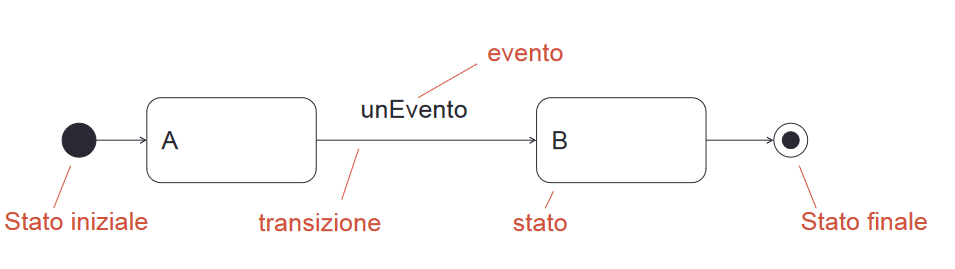
\includegraphics[scale=0.5, width=100mm]{img/macchina_a_stati_syntax.png}
\end{center}
\subsection*{Stati}
Una condizione o una situazione della vita di un oggetto durante la quale tale oggetto soddisfa
una condizione, esegue un'attività o aspetta un evento.
Lo stato di un oggetto in qualsiasi momento è determinato da
\begin{itemize}
    \item I valori dei suoi attributi
    \item Le relazioni che ha con altri oggetti
    \item Le attività che sta eseguendo
\end{itemize}
Le azioni sono istantanee e non interrompibili, le transizioni interne occorrono dentro
lo stato e non causano la transizione in un nuovo stato, mentre le attività richiedono un
intervallo di tempo finito e sono interrompibili.
\\ Le transizioni possono essere collegate tramite uno pseudo stato
di giunzione o tramite uno pseudo stato di selezione (tipo if else).
\subsection*{Eventi}
Gli \textbf{eventi} attivano le transizioni nelle macchine a stati.
\\ Ci sono eventi di diversa tipologia:
\paragraph*{Eventi di chiamata} Una chiamata per una specifica operazione.
L'evento dovrebbe avere la stessa segnatura di un'operazione della classe di contesto.
\paragraph*{Eventi di segnale} Un segnalte è un pacchetto di informazioni inviato in modo
asincrono tra oggetti. Non ha operazioni perchè il suo scopo è trasportare informazioni.
\paragraph*{Ricezione del segnale} indicata da un pentagono concavo.
\paragraph*{Evento di Variazione} Un evento di variazione è un'espressione booleana:
L'azione viene eseguita quando il valore dell'espressione passa da falso a vero.
Da un punto di vista implementativo, l'espressione viene valutata in modo periodico (ciclo di test continuo).
\paragraph*{Evento temporale} Un evento temporale è un evento che si verifica dopo un certo periodo di tempo,
quindi quando un'espressione di tempo diventa vera.
\subsection*{Stati composti}
Hanno una o più regioni ognuna delle quali contiene una sottomacchina annidata.
\\ Il più semplice contiene una sola regione, mentre quelli compositi ortogonali hanno
due o più regioni e quando si entra nello stato composito tutte le macchine iniziano la loro esecuzione
in modo concorrente. L'uiscta può essere sincronizzata, cioè si esce dallo stato quando tutte le regioni sono
terminate, oppure asincrona, cioè si esce dallo stato composito quando una regioen termina e l'altra
sottomacchine viene terminata.
\subsection*{Comunicazione tra sotto macchine}
Capita spesso di avere l'esigenza di far comunicare due sotto-macchine, biforcazioni e
ricongiuizioni possono essere usate per creare sotto-macchine concorrenti e per ri-sincronizzarle.
La comunicazione asincrona è ottenuta da una sotto-macchina configurando un flag per un'altra sotto-macchina.
\paragraph*{Stato di sync} Come alternativa all'utilizzo degli attributi possiamo utilizzare uno stato di sync
il cui compito è quello di tenere traccia di ogni singola attivazione della sua unica transizione di
input. Lo stato di sync è come se fosse una coda dove si aggiunge un elemento alla coda ogni volta
che viene attiva la transizione di input.
\subsection*{Stati con memoria semplice} 
Lo pseudo-stto con memoria semplice ricorda in quale sottostato si era quando si è lasciato il super stato,
in seguito quando si ritorna da uno stato esterno allo stato con memoria, l'indicatore ridirezione la 
transizione sull'ultimo sottostato memorizzato.
\paragraph*{Memoria multilivello} Uno stato con memoria multilivello può ricordarsi di più sottostati.
\section{I diagrammi di macchina in UP}
Non esiste nessun modello in UP chiamato "modello a stati", tuttavia qualsiasi elemento in qualsiasi modello
può avere una macchina a stati per comprendere o comunicare meglio il proprio comportamento dinamico.
\paragraph*{Esempio} Macchina a stati per rappresentare un processo di vendita, dalla selezione dell'item,
al pagamento.
\chapter{Diagramma di attività}


\end{document}